\chapter{Exercise \arabic{excounter}}
\addtocounter{excounter}{1}

\steps{Getting things started}{
\item Install \protege.
\item Install the matrix plugin.
\item Open a new ontology called \texttt{fhkb-x.owl}, where x is your student user id.
\item Remember to save your file often while working\ldots
}

\section{Installing \protege}
Go to \url{http://protege.stanford.edu/download/registered.html} and download the platform independent installer of \protege Desktop 4.X (you do not have to register in order to download the software). Select the appropriate one for your operating system. We recommend downloading it bundled with the Java VM, to ensure compatibility. After the download is completed, run the installer and follow the instructions, selecting the appropriate VM (either the one bundled with it or your default one). 

Once the installation is completed, open \protege and go to File >> Check for plugins. Select the Matrix views plugin, as shown on the screenshot towards the end of this chapter. Click install, wait until the software asks for a restart, close and re-open \protege. Use this plugin when you need to add lots of assertions on individuals etc.

\section{Create a first ontology}
Select File >> Save as, select either RDF/XML or OWL/XML, navigate to your preferred directory and save the file using the name fhkb. The extension (*.owl) is put automatically. To be sure, go to File >> Save, and do so frequently during your upcoming modelling efforts, as \protege is known to crash in the unlikeliest situations.

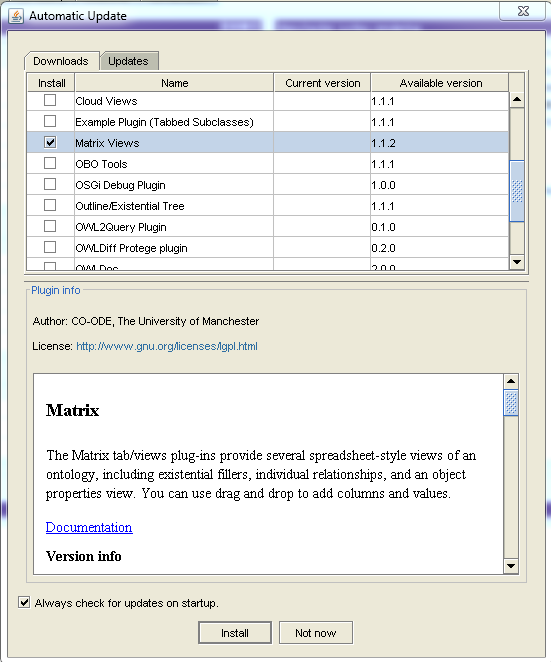
\includegraphics[width=15cm]{images/matrix_install.PNG}